% \usepackage{amsmath,amsfonts,amssymb,mathrsfs}
% \usepackage{graphicx}
% \usepackage{psfrag,graphicx,epsfig,epsf}
% \usepackage[ruled,linesnumbered, noend]{algorithm2e}
% \usepackage{fancyhdr}
% \usepackage{wrapfig}
% \usepackage{subfigure}
% \usepackage{mathtools}
% \usepackage{url}
% \usepackage{color}
% \usepackage{verbatim}
% \usepackage{xspace}

% \DeclareMathOperator*{\argmin}{arg\,min}

% \newcommand\permu[2][^n]{\prescript{#1\mkern-2.5mu}{}P_{#2}}
% \newcommand\combi[2][^n]{\prescript{#1\mkern-0.5mu}{}C_{#2}}


% \begin{document}

% \title{Fast High-Quality Dual-Arm Rearrangement in Synchronous, Monotone Tabletop Setups: Appendix}
% %\titlerunning{Fast Methods for Synchronized Tabletop Dual-Arm Rearragement}
% \author{Rahul Shome$^1$ \and Kiril Solovey$^2$ \and Jingjin Yu$^1$ \and Kostas Bekris$^1$ \and Dan Halperin$^2$}
% %\authorrunning{Shome et al.}
% \institute{$^1$Rutgers University, NJ, USA and $^2$Tel Aviv University, Israel}


% \maketitle
% \newcommand{\danh}[2][1=]{\todo[linecolor=blue,
			backgroundcolor=blue!5,bordercolor=black,#1]{DH:#2}}
\newcommand{\kb}[2][1=]{\todo[linecolor=green,
			backgroundcolor=green!5,bordercolor=black,#1]{KB:#2}}
\newcommand{\ks}[2][1=]{\todo[linecolor=red,
			backgroundcolor=red!5,bordercolor=black,#1]{KS:#2}}
\newcommand{\rs}[2][1=]{\todo[linecolor=orange,
			backgroundcolor=orange!10,bordercolor=black,#1]{RS:#2}}
\newcommand{\jy}[2][1=]{\todo[linecolor=black,
			backgroundcolor=black!5,bordercolor=black,#1]{JJ:#2}}

%%% Mathematical Definitions
\newcommand{\reals}{\mathbb{R}}
\newcommand{\integers}{\mathbb{Z}}

%%% Definitions for Workspace, Objects, Manipulator
\newcommand{\Wspace}{\mathcal{W}}
\newcommand{\Objects}{\mathcal{O}}
\newcommand{\Manip}{\mathcal{M}}
\newcommand{\nobj}{k}

%% Definitions for Object stuff
\newcommand{\Pspace}{\mathcal{P}}
\newcommand{\Pstable}{\mathcal{P}^s}
\newcommand{\pose}{p}
\newcommand{\GeomObj}{\mathcal{WO}}
\newcommand{\Arrange}{\mathcal{A}}
\newcommand{\Pumped}{\mathcal{A^P}}
\newcommand{\pumpedarr}{\alpha^{\mathcal{P}}}

%% Definitions for Manipulator stuff
\newcommand{\Qspace}{\mathcal{Q}}
\newcommand{\GeomManip}{\mathcal{WM}}

%% Definitions for problem and state space
\newcommand{\Tspace}{\mathbb{T}} 
\newcommand{\Xspace}{\mathbb{X}}
\newcommand{\paths}{\Pi}

%% Manipulation roadmap definition
\newcommand{\roadmap}{\mathcal{R}}
\newcommand{\graph}{\mathcal{G}}
\newcommand{\nodes}{\mathcal{V}}
\newcommand{\node}{{v}}
\newcommand{\edges}{\mathcal{E}}
\newcommand{\edge}{{e}}
\newcommand{\prmstar}{{\tt PRM$^*$}}

\newcommand{\rpg}{${\tt RPG}$}

\newcommand{\local}{\mathcal{L}}

\newcommand{\prm}{{\tt PRM}}
\newcommand{\kprmstar}{{\tt k-PRM$^*$}}
\newcommand{\rrt}{{\tt RRT}}
\newcommand{\rrtdrain}{{\tt RRT-Drain}}
\newcommand{\rrg}{{\tt RRG}}
\newcommand{\est}{{\tt EST}}
\newcommand{\rrtstar}{{\tt RRT$^*$}}
\newcommand{\srrt}{{\tt RDG}}
\newcommand{\bvp}{{\tt BVP}}
\newcommand{\rdg}{{\tt RDG}}
\newcommand{\lrg}{{\tt LRG}}
\newcommand{\alg}{{\tt ALG}}
\newcommand{\upump}{{\tt UPUMP}}
\newcommand{\prxpump}{{\tt RPG}}
\newcommand{\fixed}{{\tt Fixed}-$\alpha$-\rdg}
\newcommand{\nrob}{k}
\newcommand{\cons}{K}

\newcommand{\frnodes}{V_f}
\newcommand{\frnode}{v_f}
\newcommand{\grnodes}{V_g}
\newcommand{\grnode}{v_g}
\newcommand{\fredges}{E_f}
\newcommand{\fredge}{e_f}
\newcommand{\gredges}{E_g}
\newcommand{\gredge}{e_g}
\newcommand{\kedges}{E_{\cons}}
\newcommand{\kedge}{e_{\cons}}
\newcommand{\safe}{q_s^{\mathcal{M}}}
\newcommand{\hedges}{E_H}
\newcommand{\hedge}{e_H}
\newcommand{\hnodes}{V_H}
\newcommand{\hnode}{v_H}
\newcommand{\hgraph}{H}
\newcommand{\nblank}{b}
\newcommand{\config}{C}
\newcommand{\cquery}{\mathbb{C}}
\newcommand{\pumped}{P}
\newcommand{\pumpedgraph}{\mathcal{G}_P}
\newcommand{\pnodes}{V_P}
\newcommand{\pnode}{v_P}
\newcommand{\pedges}{E_P}
\newcommand{\pedge}{e_P}
\newcommand{\signs}{\Sigma}
\newcommand{\sign}{\sigma}
\newcommand{\gsign}{\sigma_{\pumpedgraph}}
\newcommand{\cedges}{E_c}
\newcommand{\constraints}{\tt c}


\newenvironment{myitem}{\begin{list}{$\bullet$}
{\setlength{\itemsep}{-0pt}
\setlength{\topsep}{0pt}
\setlength{\labelwidth}{0pt}
%\setlength{\labelsep}{0pt}
\setlength{\leftmargin}{10pt}
\setlength{\parsep}{-0pt}
\setlength{\itemsep}{0pt}
\setlength{\partopsep}{0pt}}}%
{\end{list}}

%\newtheorem{theorem}{Theorem}
%\newtheorem{definition}[theorem]{Definition}
%\newtheorem{proposition}[theorem]{Proposition}
%\newtheorem{corollary}[theorem]{Corollary}
%\newtheorem{axiom}[theorem]{Axiom}
% \newtheorem{lemma}[theorem]{Lemma}
%\newtheorem{problem}{Problem}
%\newtheorem{prob}[theorem]{Problem}
%\newtheorem{conjecture}[theorem]{Conjecture}
%\newtheorem{obj}[theorem]{Objective}
%\newtheorem{prop}[theorem]{Property}
%\newtheorem{schedule}[theorem]{Schedule}

\newtheorem{thm}{Theorem}
\newtheorem{lemma}[thm]{Lemma}
\newtheorem{definition}[thm]{Definition}


%\newtheorem{definition}{\bf Definition}
%\newtheorem{assumption}{\bf Assumption}
%\newtheorem{thm}{\bf Theorem}
%\newtheorem{requirement}{\bf Requirement}
%\newtheorem{lemmma}{\bf Lemma}
%\newtheorem{coro}{\bf Corollary}





%%%%%%%%%%%%%%%%%%%%%%%%%%%%%%%%%%%%
%% Nick Saving space
%%%%%%%%%%%%%%%%%%%%%%%%%%%%%%%%%%%%
% Space between figure and caption
%\setlength{\abovecaptionskip}{-2.5pt}
%\setlength{\belowcaptionskip}{-6pt}
%% Space between text and figs
%\setlength{\dbltextfloatsep}{2pt plus 1.0pt minus 1.0pt}
%\setlength{\textfloatsep}{2pt plus 1.0pt minus 1.0pt}
%\setlength{\intextsep}{2pt plus 1.0pt minus 1.0pt}
%% Space between equations and text
%\setlength{\belowdisplayskip}{0pt} \setlength{\belowdisplayshortskip}{2pt}
%\setlength{\abovedisplayskip}{0pt} \setlength{\abovedisplayshortskip}{2pt}

\newcommand{\dof}{{\tt DoF}}

\newcommand{\mam}{$\mathcal{G}_{\tt MAM}$}
\newcommand{\pr}{\ensuremath{\mathbb{P}}}


\newcommand{\rad}{\ensuremath{r(n)}}
\newcommand{\radstar}{\ensuremath{r^*(n)}}
\newcommand{\radi}{\ensuremath{r_i(n)}}
\newcommand{\radj}{\ensuremath{r_j(n)}}
\newcommand{\crossrad}{\ensuremath{r_R(n)}}
\newcommand{\crossradstar}{\ensuremath{r^*_R(n)}}
\newcommand{\impcrossrad}{\ensuremath{\hat r_R(n)}}
\newcommand{\allimpcrossrad}{\ensuremath{\hat r_{R}(n^R)}}
\newcommand{\ki}{\ensuremath{k_i(n)}}
\newcommand{\kj}{\ensuremath{k_j(n)}}

%% Manipulation roadmap definition
\newcommand{\mmgraph}{\ensuremath{\mathbb{G}}}
\newcommand{\mmgimp}{\hat\mmgraph}
\newcommand{\mmgexp}{\mmgraph}
\newcommand{\aograph}{\ensuremath{\mathbb{G}^{AO}}}
\newcommand{\tree}{\ensuremath{\mathbb{T} \ }}
\newcommand{\mmnodes}{\mathbb{\hat V}}
\newcommand{\mmedges}{\mathbb{\hat E}}
\newcommand{\mmnodestpprm}{\mathbb{V}_{\chi_i}}
\newcommand{\mmedgestpprm}{\mathbb{E}_{\chi_i}}
\newcommand{\mmnode}{\mathbb{\hat v}}
\newcommand{\mmedge}{\mathbb{\hat e}}
\newcommand{\sprmstar}{Soft-\ensuremath{ {\tt PRM} }}
\newcommand{\irs}{\ensuremath{ {\tt IRS} }}
\newcommand{\spars}{{\tt SPARS}}
\newcommand{\drrt}{\ensuremath{{\tt dRRT}}}
\newcommand{\drrtstar}{\ensuremath{{\tt dRRT^*}}}
\newcommand{\dadrrtstar}{\ensuremath{\tt da\_dRRT^*}}

\newcommand{\sig}{{\tt SIG}}
\newcommand{\rmaps}{\ensuremath{\mathfrak{R}}}

\newcommand{\mmprm}{\ensuremath{\text{Random-}{\tt MMP}}}
\newcommand{\astar}{{\ensuremath{\tt A^{\text *}}}}
\newcommand{\mstar}{{\tt M^{\text *}}}
\newcommand{\opens}{P_{Heap}}


\newcommand{\cost}{\textup{cost}}



%\newcommand*{\qed}{\hfill\ensuremath{\square}}

\newcommand{\kiril}[1]{{\color{blue} \textbf{Kiril:} #1}}
\newcommand{\chups}[1]{{\color{green} \textbf{Chuples:} #1}}
\newcommand{\rahul}[1]{{\color{red} \textbf{Rahul:} #1}}

\newcommand{\T}{\mathcal{T}}

% Dual Arm
\newcommand{\leftrm}{\ensuremath{\mathbb{R}_{l}}  }
\newcommand{\rightrm}{\ensuremath{\mathbb{R}_{r}}  }
\newcommand{\leftmetric}{\ensuremath{\mathbb{P}_{l}}  }
\newcommand{\rightmetric}{\ensuremath{\mathbb{P}_{r}}  }
\newcommand{\cfull}{\ensuremath{\mathbb{C}_{{\rm full}}}  }
\newcommand{\cfree}{\ensuremath{\mathbb{C}_{{\rm free}}}  }
\newcommand{\cobs}{\ensuremath{\mathbb{C}_{{\rm obs}}}  }
\newcommand{\cleft}{\ensuremath{\mathbb{C}_{{l}}}  }
\newcommand{\cright}{\ensuremath{\mathbb{C}_{{r}}}  }
\newcommand{\cshared}{\ensuremath{\mathbb{C}_{{s}}}  }
\newcommand{\cgoal}{\ensuremath{q_{{\rm goal}}}  }
\newcommand{\cstart}{\ensuremath{q_{{\rm start}}}  }

\newcommand{\gimpleft}{\ensuremath{\hat\mmgraph_l}}
\newcommand{\gimpright}{\ensuremath{\hat\mmgraph_r}}


\newcommand{\xrand}{\ensuremath{x^{\textup{rand} \ }}}
\newcommand{\xnear}{\ensuremath{x^{\textup{near} \ }}}
\newcommand{\xnew}{\ensuremath{x^{\textup{n}} \ }}
\newcommand{\xlast}{\ensuremath{x^{\textup{last} \ }}}
\newcommand{\xparent}{\ensuremath{x^{\textup{best} \ }}}

\newcommand{\lr}{\ensuremath{\mathbb{R}_{ls}}}
\newcommand{\rr}{\ensuremath{\mathbb{R}_{sr}}}
\newcommand{\lp}{\ensuremath{\mathbb{P}_{l}}}
\newcommand{\rp}{\ensuremath{\mathbb{P}_{r}}}

\newcommand{\motoman}{{\tt Motoman}}
\newcommand{\baxter}{{\tt Baxter}}
\newcommand{\ao}{{\tt AO}}

\newcommand\inlineeqno{\stepcounter{equation}\ (\theequation)}

\newcommand{\chomp}{\ensuremath{\tt CHOMP } }

\newtheorem{assumption}{Assumption}

\newcommand{\W}{\mathcal W}
\newcommand\perm[2][\^n]{\prescript{#1\mkern-2.5mu}{}P\_{#2}}
\newcommand\comb[2][\^n]{\prescript{#1\mkern-0.5mu}{}C\_{#2}}
\newcommand{\objectset}{\mathcal{O}}
\newcommand{\object}{o}
\newcommand{\workspace}{\mathcal{W}}
\newcommand{\taskspace}{\mathcal{T}}
\newcommand{\arrangement}{A}
\newcommand{\oar}{p}
\newcommand{\manipulators}{\mathcal{M}}
\newcommand{\manipulator}{\mathit{m}}
\newcommand{\arm}{m}
\newcommand{\taskset}{\mathcal{T}}
\newcommand{\task}{\mathit{T}}
\newcommand{\sol}{\Pi}
\newcommand{\state}{q}

\newcommand{\Aspace}{\mathcal{A}}
\newcommand{\Afree}{\mathcal{A}_{\rm val}}
\newcommand{\ainit}{A_{\rm init}}
\newcommand{\atarget}{A_{\rm goal}}
\newcommand{\soma}{{\tt soma}}
\newcommand{\coma}{\ensuremath{{\omega}}}
\newcommand{\scoma}{\ensuremath{{{\Omega}}}}
\newcommand{\qset}{\mathcal{Q}}
\newcommand{\startq}{S}
\newcommand{\targetq}{T}

\newcommand{\act}{a}
\newcommand{\actset}{\mathbb{A}}
\newcommand{\trajset}{{\D}}
\newcommand{\moveset}{\bar{\mathcal{O}}}
\newcommand{\home}{Q}
\newcommand{\scomaset}{\{\scoma\}}
\newcommand{\tour}{{\Gamma}}
\newcommand{\tspgraph}{\graph_{\tour}}
\newcommand{\tspnodes}{\nodes_{\tour}}
\newcommand{\tspedges}{\edges_{\tour}}
\newcommand{\algo}{{\tt{TOM}}\xspace}
\newcommand{\kuka}{{\tt{Kuka }}}
\newcommand{\D}{D}
\newcommand{\sininv}{\sin^{-1}}
\newcommand{\cosinv}{\cos^{-1}}
\newcommand{\milp}{{\tt{MILP}}\xspace}
%%%%%%%%%%%%%%%%%%%%%%%%%%%%%%
%Caption model
\newcounter{model}
%\addtocounter{model}{1}
\newenvironment{model}
{\refstepcounter{model}}
{\begin{center}
\textbf{Model. }~\themodel
\end{center}
\medskip}
%%%%%%%%%%%%%%%%%%%%%%%%%%%%%%
\definecolor{darkgreen}{RGB}{30,150,30}
% \newcommand{\commentdel}[1]{{\color{magenta} #1}}
\newcommand{\commentdel}[1]{{\color{magenta}}}
%\newcommand{\commentadd}[1]{{\color{darkgreen} #1}}
 \newcommand{\commentadd}[1]{{#1}}
 \newcommand{\cameraready}[1]{{ #1}}
%  \newcommand{\cameraready}[1]{{#1}}
\newcommand{\tase}[1]{{\color{darkgreen} #1}}


\newcommand\blfootnote[1]{%
  \begingroup
  \renewcommand\thefootnote{}\footnote{#1}%
  \addtocounter{footnote}{-1}%
  \endgroup
}
% \documentclass{llncs}

%####################################################################################
%####################################################################################
%####################################################################################
%####################################################################################
%####################################################################################


\subsection{Expected k-arm cost bounds in a planar disk manipulator model}
\commentadd{
The arguments made in Theorem \ref{thm:karm} can be extended to $k$ disc arms.
In the planar unit-square setting, with $k$ arms, there are $\frac{n}{k}$ objects 
for each arm to work with. Consider the transfers and transits of a set of $k$ 
objects, one for each arm. By \cite{ChiHanYu2018WAFR}, the arbitrary rearrangement of $k$ discs 
can be achieved in a bounded region with a perimeter of $O(kr)$. 
Clearly, the per robot additional (makespan or distance) cost is bounded by some 
function $f(k, r)c_t$, which goes to zero as $r$ goes to zero. Adding up all the potential 
extra cost,  a $k$-arm solution has a cumulative cost

{\centerline
{
$C_{\rm k{\text-}arm} = C_{\rm single} + nf(k,r)c_t \approx (c_{pd} + 0.52c_t + f(k,r)c_t)n\;.$
}
}

\noindent For fixed $k$ and small $r$, $C_{\rm k{\text-}arm}$ is almost the same as $C_{\rm single}$.
%, $c_t$ is a distance (e.g., energy) cost. 
Upon considering the maximum of the two arc lengths or makespan,
the $k$-arm cost becomes $C_{\rm k{\text-}arm}^t \approx (c_{pd} + 0.52c_t)\frac{n}{k} + nf(k,r)c_t$.

The cost ratio is
\vspace{-0.1in}
\begin{equation}\label{eq:kmakespan-ratio}
\frac{C_{\rm k{\text-}arm}^t}{C_{\rm single}} \approx 
\frac{(c_{pd} + 0.52c_t)\frac{n}{k} + nf(k,r)c_t}{(c_{pd} + 0.52c_t)n}
= \frac{1}{k} + \frac{f(k,r)c_t}{c_{pd} + 0.52c_t}\;.
% \vspace{-0.1in}
\end{equation}

When $r$ is small or when $\frac{c_t}{c_{pd}}$ is small, the $k$-arm 
solution is roughly $\frac{1}{k}$ as costly as the single arm solution. On 
the other hand, in this model a $k$-arm solution does not do better than $\frac{1}{k}$ of 
the single arm.

\begin{theorem}
For rearranging objects with non-overlapping starts and goals that are
uniformly distributed in a unit square,  a $k$-arm solution can have an 
asymptotic improvement of $\frac{1}{k}$ over the single arm solution. 
\end{theorem}
}
% \rahul{Need to verify this line of reasoning}


\subsection{Expected measure of the maximum of lengths of two random lines on an unit square}
Prior work \cite{ghosh1951random} defines the \textit{pdf} of lengths($l$) of randomly sampled lines in a rectangle of sides $a,b, \ \ a\geq b$ as 
\begin{align*}
p(l) &= (\frac{4l}{a^2b^2})\phi(l)\\
\phi(l)&= \frac{1}{2}\pi a b - a l - b l + \frac{1}{2} l^2, \ \ l\in[0,b]\\
\phi(l)&= ab \sininv(\frac{b}{l}) + a. \sqrt[]{(l^2-b^2)} - al - \frac{1}{2}b^2, \ \ l\in[b,a]\\
\phi(l)&= ab\{\sininv(\frac{b}{l})-\cosinv(\frac{a}{l})\} + a\sqrt[]{(l^2-b^2)} + b\sqrt[]{(l^2-a^2)} \\
&- \frac{1}{2}(l^2+a^2+b^2),\ \ l\in[a,\sqrt[]{(a^2+b^2)}]
\end{align*}

In the unit square model, $a=b=1$. Substituting the values, the \textit{pdf} becomes
\begin{align}
p(l)&= 2\pi l - 8\pi l^2 + 2l^3, \ \ l\in[0,1]\\
p(l)&= 4l\sininv(\frac{1}{l}) - 4l\cosinv(\frac{1}{l}) + 8l\sqrt[]{(l^2-1)} -2l^3 -4l, \ \ l\in[1,\sqrt[]{2}]
\end{align}

Assuming two random sets of lines, representing transfers in a random split of objects between two arms, we need the expected value of the maximum of these pairwise lengths ie., $\mathtt{E}(max(l_1,l_2)), \ \ l_1,l_2\ i.i.d, \ \ l_1 \sim p, l_2 \sim p$.
This is estimated using the \textit{pdf} obtained. 
\begin{equation}
\mathtt{E}(max(l_1,l_2)) = \int_0^{\sqrt[]{2}} \int_0^{\sqrt[]{2}} max(l_1,l_2)p(l_1)p(l_2) dl_2 dl_1 \approx 0.663
\end{equation}
The result is calculated by taking into account the combination of different ranges of $p(l)$ and $max(l_1,l_2)$.
\commentadd{
\begin{wrapfigure}{r}{1.4in}
	\centering
	\vspace{-0.3in}
    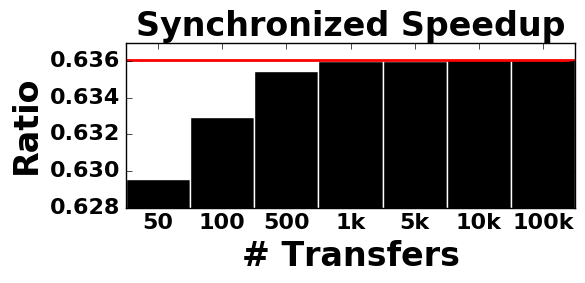
\includegraphics[width=1.4in]{figures/monte_carlo}
	\caption{Empirical cost ratio versus the estimate}
  	\label{fig:bounds}
\end{wrapfigure}

Prior work~\cite{santalo2004integral} offered an estimate for the expected length of a transit path $C_{sg}$ in terms of the expected length of a line segment, $0.52$, in a randomized setting in an unit square. With the current estimate of $0.663$ for the maximum of two such randomly sampled line segments, it follows that, the expected makespan or maximum of distances cost will use this estimate.

Using this result, the synchronized cost ratio is stated in Equation~\ref{eq:synchronized-ratio} as
$$
\frac{C_{\rm dual}^{\rm sync}}{C_{\rm single}} \approx 
\frac{(c_{pd} + 0.66c_t)\frac{n}{2} + 4n\pi rc_t}{(c_{pd} + 0.52c_t)n}
$$
As a way to validate our asymptotic estimate, randomized trials were run with different number randomly sampled object transfer coordinates on an unit square.
% Fig \ref{fig:bounds} verifies empirically that the ratio of $\frac{C_{dual}^{sync}}{C_{single}}$ when $c_{pd}=0,r=0$, asymptotically converges to the calculated expected value of $0.636$. 
When $c_{pd}=0$ and $r=0$, the ratio of $\frac{C_{dual}^{sync}}{C_{single}}$ evaluates to $0.636$. Fig \ref{fig:bounds} verifies empirically that the ratio converges to the expected value as the number of transfers increases.
This indicates the asymptotic speedup of a synchronized dual arm solution for a makespan or maximum of distances cost metric.
}

\subsection{Smoothing}
The result of the velocity tuning over the solution trajectories for the individual arms as a post-processing step is shown in Fig \ref{fig:smoothing}. The objective is to minimize any waits that might be a by-product of the synchronization. 
% The small improvements indicate that synchronization does not adversely affect the solution executions. 
The small \% improvements indicate that the asynchronous variants of the solutions discovered from the methods do not yield a big enough saving in execution time. 
Most of the improvement as a percentage of the original solution duration is not too high. On top of that, the time taken to smooth the solutions for \algo (overlaid on Fig \ref{fig:smoothing}) shows that it is often not beneficial.
In their largest problem instances the \kuka spent $ 0.44s $ of smoothing time to save $ 3.23s $ off the solution duration, while the picker spent $  9.84s $ to save $ 0.54s $.
This indicates that among the class of synchronized solutions discovered by the proposed algorithms, the analogous asynchronous variants do not seem to be drastically better. Moreover, smoothing does not improve the maximum of distances cost measure, but only reduces the solution duration. The theoretical bounds in the simple planar setups agree with the results in that the synchronization does not degrade the benefits of using 2 arms too much. It should be pointed out though that it needs to be studied further, whether these trends would hold for a class of algorithms that can solve the asynchronous dual-arm rearrangement problem in general setups. This is out of the scope of the current work.
 
% \kiril{What is the bottom line here? Is smoothing worthwhile? The y-axis in the plots is labeled as \% whereas the bars are labeled with seconds.}


% \vspace{-0.2in}
\begin{figure}
	\centering
	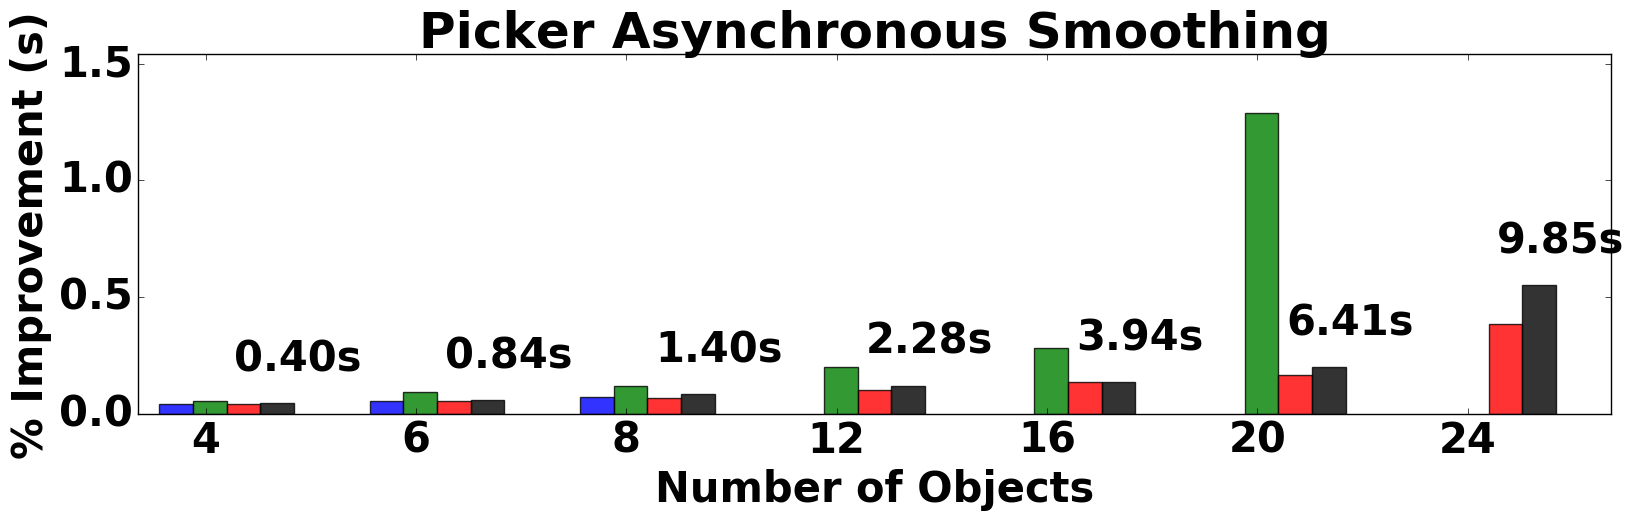
\includegraphics[width=2.3in]{figures/results/sp_smoothing}
	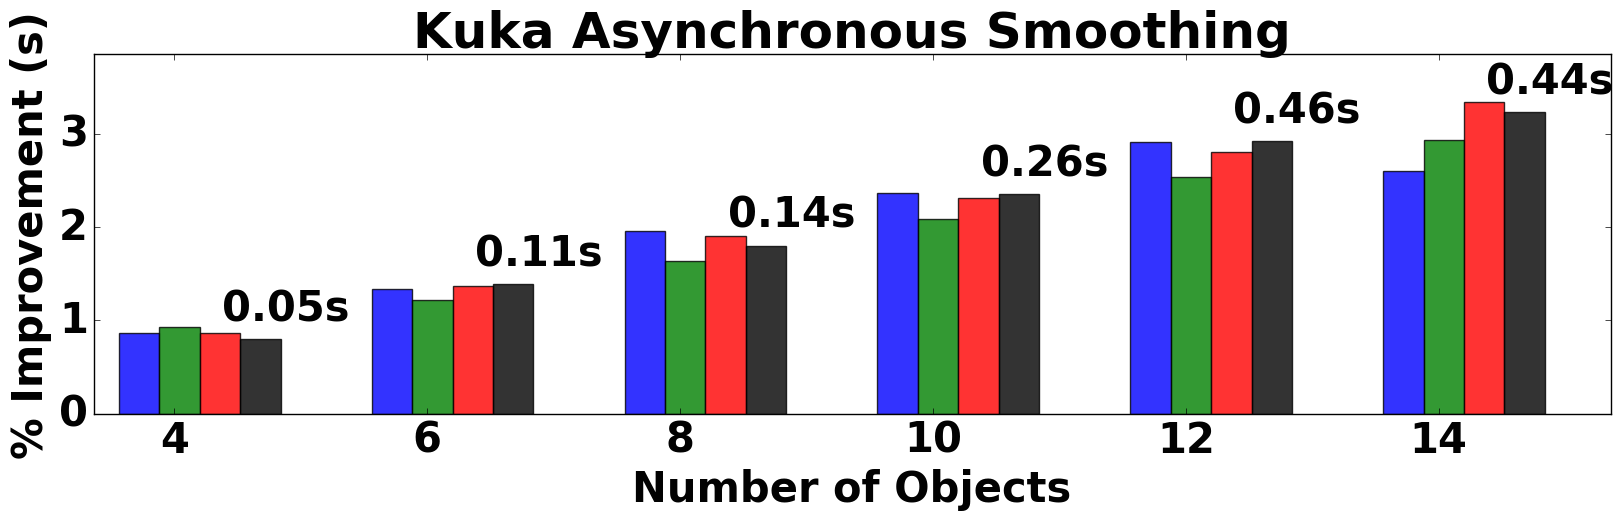
\includegraphics[width=2.3in]{figures/results/kuka_smoothing}
	\caption{Smoothed solution improvement as a percentage of the original synchronized solution duration, and the time taken to smooth solutions obtained from \algo in seconds.}
	\label{fig:smoothing}
%     \vspace{-.3in}
\end{figure}

\subsection{Discrete Reachability Benchmark}
In this benchmark, two Kuka arms are placed opposite a target arrangement table. The initial poses of the objects are set to be on opposite ends of the arms, as demonstrated in the image. The purpose of this study is to see the effects of general divided workspaces where both the initial and target poses are not in the region of common reachability of the arms. This is indeed a simpler problem for the coordinated methods, but proves challenging to the naive random split strategy. 

\begin{figure}
	\centering
	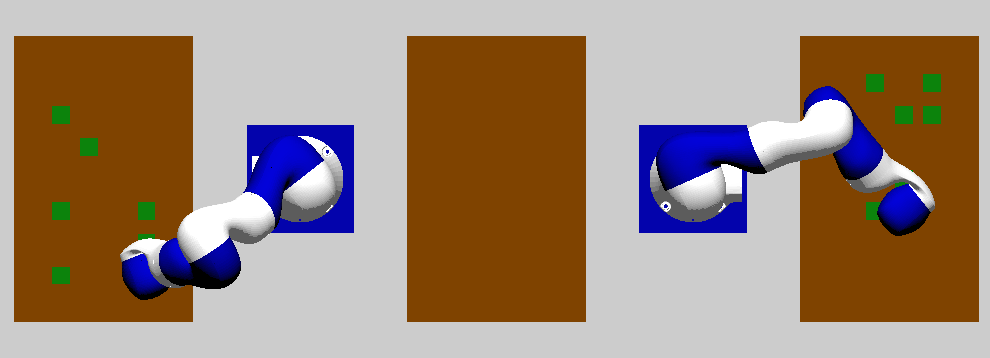
\includegraphics[width=5.3in]{figures/reachability}
	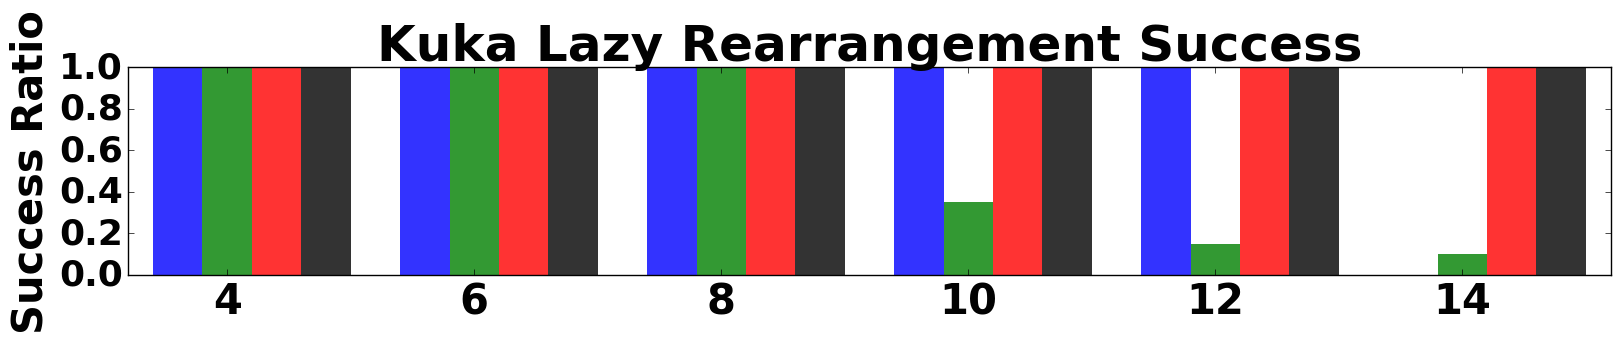
\includegraphics[width=5.3in]{figures/results/5_kuka_lazy_ms_success.png}
	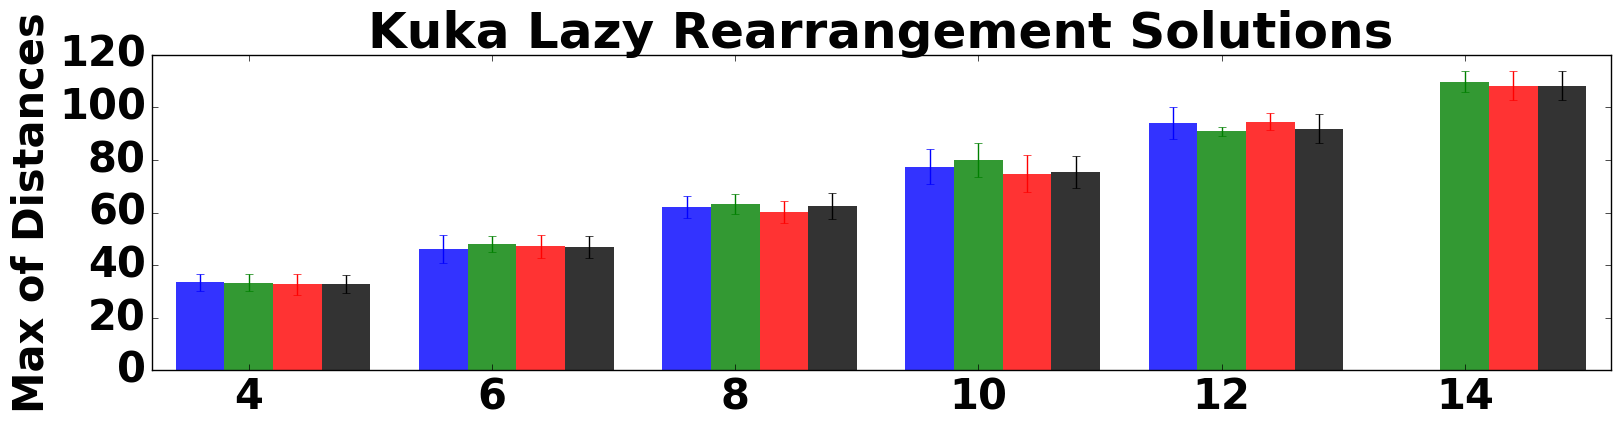
\includegraphics[width=5.3in]{figures/results/5_kuka_lazy_ms_cost.png}
	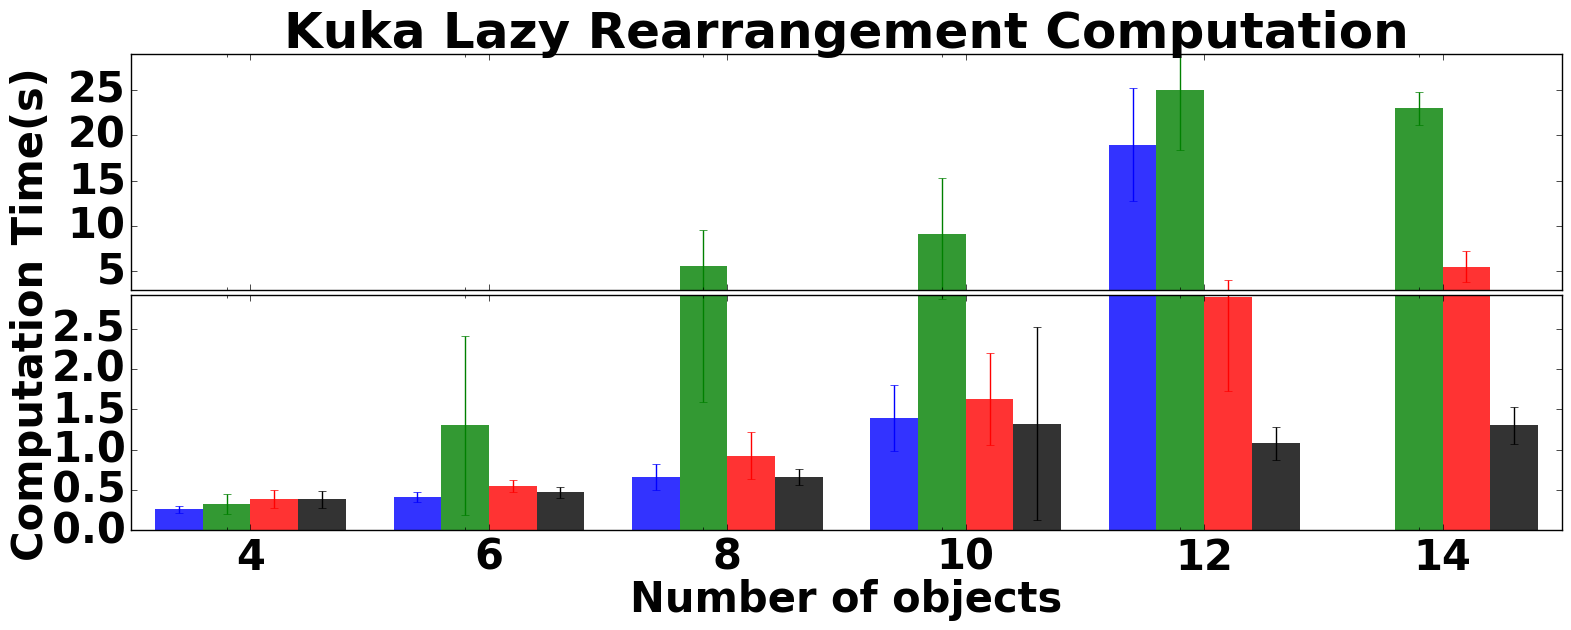
\includegraphics[width=5.3in]{figures/results/5_kuka_lazy_ms_time.png}
	\caption{The reachability benchmark}
	\label{fig:reachability_benchmark}
%     \vspace{-.3in}
\end{figure}



%####################################################################################
%####################################################################################
%####################################################################################
%####################################################################################
%####################################################################################
% {\small
% \bibliographystyle{spmpsci}
% \bibliography{bib/manip}}

% \end{document}













